\documentclass[11pt,letterpaper]{article}
\usepackage[lmargin=1in,rmargin=1in,bmargin=1in,tmargin=1in]{geometry}
\usepackage{../style}

\setlength{\parindent}{0ex}

% -------------------
% Content
% -------------------
\begin{document}

\pagenumbering{gobble}

% Recitation: Polynomials (Linear & Quadratic Functions)
\phantom{} \hfill {\bfseries \Large Recitation: Polynomials (Linear \& Quadratic Functions) Solutions} \hfill \phantom{} \par\vspace{0.5cm}

% Problem 1
\noindent {\bfseries Problem 1.} Sketch the function $f(x)= 7 - (x - 5)^2$.
	\[
	\fbox{
	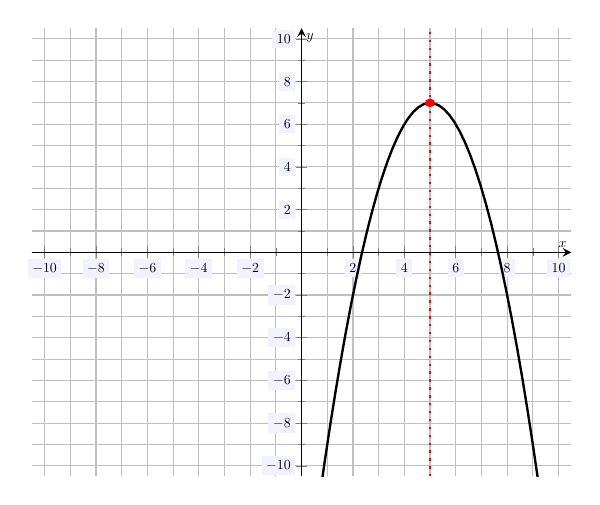
\begin{tikzpicture}[scale=1,every node/.style={scale=0.5}]
	\begin{axis}[
	grid=both,
	axis lines=middle,
	ticklabel style={fill=blue!5!white},
	xmin= -10.5, xmax=10.5,
	ymin= -10.5, ymax=10.5,
	xtick={-10,-8,-6,-4,-2,0,2,4,6,8,10},
	ytick={-10,-8,-6,-4,-2,0,2,4,6,8,10},
	minor tick = {-10,-9,...,10},
	xlabel=\(x\),ylabel=\(y\),
	]
	\addplot[line width=0.03cm,domain=-10:10,samples=100] ({x},{7 - (x - 5)^2});
	\draw[line width=0.03cm,red,dotted] (5,-10.5) -- (5,10.5);
	\draw[draw=none,fill=red] (5,7) circle (0.2);
	\end{axis}
	\end{tikzpicture}
	}
	\] \par\vspace{0.3cm}

\noindent{\itshape We know $f(x)$ has vertex $(5, 7)$, axis of symmetry $x= 5$, and opens downwards (because $a= -1 < 0$). Using this information gives us the sketch above.} \par\vspace{0.3cm}



% Problem 2
\noindent {\bfseries Problem 2.} Find the equation of the quadratic function shown below. Be sure to fully justify why your answer is correct.
	\[
	\fbox{
	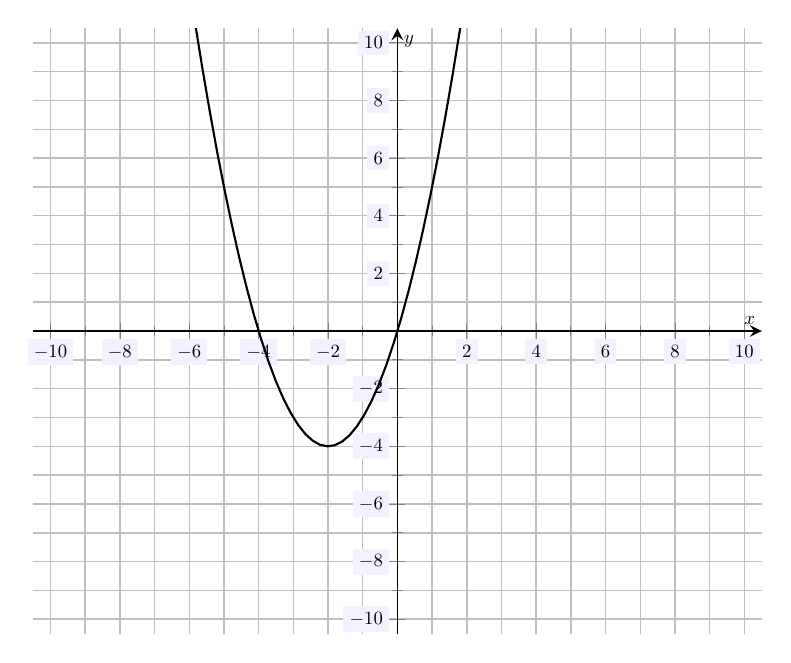
\begin{tikzpicture}[scale=1.35,every node/.style={scale=0.5}]
	\begin{axis}[
	grid=both,
	axis lines=middle,
	ticklabel style={fill=blue!5!white},
	xmin= -10.5, xmax=10.5,
	ymin= -10.5, ymax=10.5,
	xtick={-10,-8,-6,-4,-2,0,2,4,6,8,10},
	ytick={-10,-8,-6,-4,-2,0,2,4,6,8,10},
	minor tick = {-10,-9,...,10},
	xlabel=\(x\),ylabel=\(y\),
	]
	\addplot[line width= 0.02cm,samples=100,domain= -10.5:10.5] ({x},{(x + 2)^2 - 4});
	\end{axis}
	\end{tikzpicture}
	}
	\] 

\noindent{\small\itshape By the Fundamental Theorem of Algebra, we know the quadratic above is $a(x - r_1)(x - r_2)$, where the $r_i$ are the roots. We see this quadratic has roots $x= -4, 0$. So, the quadratic is $a \big(x - (-4) \big)(x - 0)= ax (x + 4)$. But we see this parabola also contains the points $(-5, 5), (-2, -4), (1, 5)$. Using, for example, $(1, 5)$, we know $y= 5$ when $x= 1$, but then $5= a \cdot 1(1 + 4)$, i.e. $5= 5a$. Therefore, $a= 1$. So, the quadratic is $x(x + 4)$. \par\vspace{0.5cm}

Alternatively, we know the quadratic has the (vertex) form $a(x - P)^2 + Q$, where $(P, Q)$ is the vertex. We see this has vertex $(-2, -4)$. So, the quadratic is $a \big(x - (-2) \big)^2 - 4= a(x + 2)^2 - 4$. But we see this parabola also contains the points $(-5, 5), (-4, 0), (0,0), (1, 5)$. Using, for example, $(0, 0)$, we know $y= 0$ when $x= 0$. But then $0= a(0 + 2)^2 - 4$, so that $4a= 4$, i.e. $a= 1$. Therefore, the quadratic is $(x + 2)^2 - 4$.}



\newpage



% Problem 3
\noindent {\bfseries Problem 3.} Solve the following equation:
	\[
	5\sqrt{2}\, x + 8= -3(1 - 2x)
	\] 
	
	\[
	\begin{gathered}
	5\sqrt{2}\, x + 8= -3(1 - 2x) \\[0.3cm]
	5 \sqrt{2}\,x + 8= -3 + 6x \\[0.3cm]
	5 \sqrt{2}\,x - 6x= -11 \\[0.3cm]
	(5 \sqrt{2}\, - 6)x= -11 \\[0.3cm]
	x= \dfrac{-11}{5 \sqrt{2} - 6} 
	\end{gathered}
	\] \par\vspace{3cm}



% Problem 4
\noindent {\bfseries Problem 4.} Consider the quadratic function $f(x)= x^2 - 6x + 14$.
	\begin{enumerate}[(a)]
	\item Find $a, b, c$ for this quadratic function.
	\item Does $f(x)$ open upwards or downwards? Explain.
	\item Is this quadratic function convex or concave? Explain. 
	\item Find the minimum value of $f(x)$, if it exists. If it does not exist, explain why.  
	\item Find the maximum value of $f(x)$, if it exists. If it does not exist, explain why. 
	\end{enumerate} \par\vspace{0.5cm}

\noindent{\bfseries Solution.}
{\itshape
	\begin{enumerate}[(a)]
	\item We have $a= 1$, $b= -6$, $c= 14$.
	\item Because $a= 1 > 0$, the quadratic function opens upwards.
	\item Because $a= 1 > 0$, the quadratic function is convex. 
	\item Because $a= 1 > 0$, the quadratic function has a minimum value---namely, the $y$-coordinate of the vertex. Completing the square, we have $x^2 - 6x + 14= x^2 - 6x + 9 - 9 + 14= (x - 3)^2 + 5$. So, the minimum possible output is $5$. Alternatively, using the evaluation method, we know the minimum occurs at $x= -\tfrac{b}{2a}= -\tfrac{-6}{2(1)}= 3$. Then $f(3)= 3^2 - 6(3) + 14= 9 - 18 + 14= 5$.
	\item Because $a= 1 > 0$, the quadratic function has no maximum value. 
	\end{enumerate}
}

\end{document}